% !TEX root = _individual/implementation.tex

%%%%%%%%%%%%%%%%%%%%%%%%%%%%%%%%%%%%%%%%%%%%%%%%%%%%%%%%%%%%%%%%%%%%%%%%%%%%%%%%
\chapter{Low-order discretization schemes} \label{chap:implementation}

The use of anisotropic diffusion tensors is not new, nor is the search for
accurate discretizations. In this dissertation, we only consider a structured
two-dimensional Cartesian mesh, where all cells are quadrilaterals, and each
cell connects (in
the interior) to four adjacent cells through four faces, and each face is
perpendicular to one of the coordinate system axes.

Because of this simplified problem space, we need not implement the more
complex Support Operators Methods \cite{Mor1998,Run2006}. But the complexity is
not just a burden on the programmer; those methods increase the number of
unknowns and the change the structure of the resulting system of equations,
meaning longer solution times for the user. With this in mind, we seek in this
chapter to find simple but accurate methods of solving the low-order system of
equations for Anisotropic Diffusion on Cartesian meshes.

The traditional method of discretizing the \Pone\ equations is to use a
``staggered mesh'' where $\phi$ is cell-centered and $\vec{F}\vd \vec{n}$ is
stored on the edges of each cell \cite{War2003}. This approach conserves
radiation energy, but it does not conserve radiation momentum, an important
quantity when coupling with hydrodynamics codes \cite{Pom1973}.

%%%%%%%%%%%%%%%%%%%%%%%%%%%%%%%%%%%%%%%%%%%%%%%%%%%%%%%%%%%%%%%%%%%%%%%%%%%%%%%%
\section{Introduction}

Because the semi-implicit gray TRT formulation can be expressed as a
steady-state transport equation (see \S\ref{sec:bgSemiImplicit}), for
simplicity we will present these discretizations without time dependence.

The steady-state particle conservation equation is
\begin{equation}\label{eq:ssConservation}
  \grad \vd \vec{F}(\vec{x}) + \sigma_a(\vec{x}) \phi(\vec{x}) =
  Q(\vec{x})\,,\qquad \vec{x} \in V\,.
\end{equation}
The first step in a differencing scheme is to assume that the unknown
(in this case, $\phi$) is constant over a single cell, represented in
Fig.~\ref{fig:cellDiagram}. We also assume that the effective absorption cross
section $\sigma_a$ and source $Q$ are
constant over the cell, which, for TRT, means assuming the material temperature
is constant over a cell. Integrating Eq.~\eqref{eq:ssConservation} over cell
$i,j$ and using the divergence theorem gives
\begin{equation} \label{eq:ssConservationDisc}
  %\sum_{f\in \{L,R,B,T\}} \int_f \vec{n}_f \vd \vec{F} \ud A
  \Delta_{x,i} \left( F_T^y - F_B^y \right)
+ \Delta_{y,j} \left( F_R^x - F_L^x \right)
+ \Delta_{x,i}\Delta_{y,j} \sigma_{a,i,j} \phi_{i,j}
= \Delta_{x,i}\Delta_{y,j} q_{i,j}\,.
\end{equation}
Here, $F_A^b$ is the leakage (radiation flux) from cell $i,j$ through face $A$
along the $b$ axis. The methods presented in the following sections provide
different closures for the leakages in terms of the other unknowns. They all
serve to approximate the ``Fick's law'' of anisotropic diffusion,
\begin{equation}\label{eq:anisotropicFicks2d}
  \vec{F} = - \Dtens \vd \grad \phi
  = -
  \begin{bmatrix}
    D^{xx} & D^{yx} \\
    D^{xy} & D^{yy}
  \end{bmatrix}
  \begin{bmatrix}
    \tpder{\phi}{x} \\
    \tpder{\phi}{y}
  \end{bmatrix}
  = 
  \begin{bmatrix}
    - D^{xx} \tpder{\phi}{x}
    - D^{yx} \tpder{\phi}{y} \\
    - D^{yy} \tpder{\phi}{y}
    - D^{xy} \tpder{\phi}{x}
  \end{bmatrix}
  \,.
\end{equation}
Because the diffusion matrix is symmetric, $D^{yx}=D^{xy}$.

\begin{figure}[htb]
  \centering
  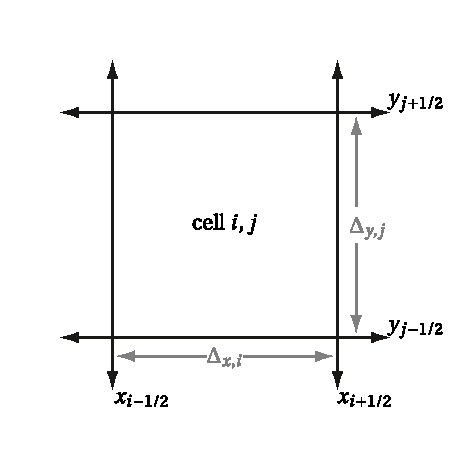
\includegraphics{cell-diagram}
  \caption{Diagram of cell $i,j$.}
  \label{fig:cellDiagram}
\end{figure}

To preserve particles, it's necessary that $F_T^y$ from cell $i,j$ is equal to
$F_B^y$ from cell $i,{j+1}$, and the same from the other directions.

%%%%%%%%%%%%%%%%%%%%%%%%%%%%%%%%%%%%%%%%%%%%%%%%%%%%%%%%%%%%%%%%%%%%%%%%%%%%%%%%
\section{Neglecting transverse diffusion}\label{sec:discreteDiag}

Perhaps the simplest way to discretize the anisotropic diffusion equation is by
neglecting the off-diagonal terms of the diffusion tensor that imply transverse
leakage.

In certain simple problems, this is not an approximation. As long as the
opacity is invariant with respect to one of the Cartesian coordinate system's
axes (see \S\ref{sec:eigenvectors}), the off-diagonal terms of $\Dtens$ are
zero, and the anisotropic Fick's law simplifies to:
\begin{equation*}
  \vec{F} = - \Dtens \vd \grad \phi
  = -
  \begin{bmatrix}
    D^{xx} & 0 \\
    0 & D^{yy}
  \end{bmatrix}
  \begin{bmatrix}
    \tpder{\phi}{x} \\
    \tpder{\phi}{y}
  \end{bmatrix}
  = 
  \begin{bmatrix}
    - D^{xx} \tpder{\phi}{x} \\
    - D^{yy} \tpder{\phi}{y}
  \end{bmatrix}
  \,.
\end{equation*}

Without loss of generality, we evaluate the net leakage from cell
$i,j$ through its right face:
\begin{align} \nonumber
  F_R^x &\equiv \frac{1}{\Delta_{y,j}} \int_{y_{j-1/2}}^{y_{j+1/2}}
  \vec{F}(x_{i+1/2}, y) \vd \vec{n}_R \ud y\,.
  \\
  \intertext{Substituting the anisotropic Fick's law,} \nonumber
  F_R^x &= - \frac{1}{\Delta_{y,j}} \int_{y_{j-1/2}}^{y_{j+1/2}}
  D_{i,j}^{xx} \pder{\phi}{x} \ud y \,.
  \\ 
  \intertext{Now we introduce a temporary cell-edge $\phi_{i+1/2}$ and
  approximate the partial derivative using a second-order finite difference:}
  \label{eq:diagFrx}
  F_R^x &\approx - 
  D_{i,j}^{xx} \frac{\phi_{i+1/2,j} - \phi_{i}}{\Delta_{x,i}/2} \,.
\end{align}
Evaluating the net leakage from cell $i+1,j$ through its left face by using the
cell-edged $\phi_{i+1/2}$ and finite difference approximation, we obtain
\begin{equation}\label{eq:diagFlx}
  F_{L,i+1,j}^x \approx - 
  D_{i+1,j}^{xx} \frac{\phi_{i+1,j} - \phi_{i+1/2}}{\Delta_{x,i+1}/2} \,.
\end{equation}
Scaling Eqs.~\eqref{eq:diagFrx} and~\eqref{eq:diagFlx} by $\Delta_x/(2 D^{xx})$
and adding them, we obtain
\begin{equation*}
  \frac{\Delta_{x_{i+1/2}}}{D_{i,j}^{xx}}F_R^x
 + \frac{\Delta_{x_{i+1/2}}}{D_{i+1,j}^{xx}}F_{L,i+1,j}^x
 = -(\phi_{i+1/2,j} - \phi_{i}) + -(\phi_{i+1,j} - \phi_{i+1/2})\,.
\end{equation*}
The cell-edged $\phi$ cancels out. Enforcing particle conservation by
setting $F_R^x = F_{L,i+1,j}^x$ yields the expression for the net leakage
through the right face of cell $i,j$:
\begin{equation}\label{eq:diagRight}
  F_R^x= -\frac{D^{xx}_{i+1/2,j}}{\Delta_{x,i+1/2}}
  \left( \phi_{i+1,j} - \phi_{i,j} \right)\,,
\end{equation}
where we have defined a harmonically averaged cell edge diffusion coefficient
and a half-edge width,
\begin{equation} \label{eq:cellEdgeDHarmonic}
  \frac{D^{xx}_{i+1/2,j}}{\Delta_{x,i+1/2}} \equiv \left[
  \frac12 \left( \frac{D^{xx}_{i,j}}{\Delta_{x,i}} \right)\inv
 + \frac12 \left( \frac{D^{xx}_{i+1,j}}{\Delta_{x,i+1}} \right)\inv
  \right]\inv\,.
\end{equation}
This is the standard relation between neighboring cells in the
cell-centered discretization scheme \cite{Dud1976}, except that in anisotropic
diffusion, leakage across the face normal to the $x$ axis takes the $D^{xx}$
component of the diffusion tensor.

Repeating the same procedure through the left, top, and bottom faces yield the
following similar equations:
\begin{align*}
  F_L^x &= -\frac{D^{xx}_{i-1/2,j}}{\Delta_{x,i-1/2}}
  \left( \phi_{i,j} - \phi_{i-1,j} \right)\,,
  \\
  F_T^y &= -\frac{D^{yy}_{i,j+1/2}}{\Delta_{y,j+1/2}}
  \left( \phi_{i,j+1} - \phi_{i,j} \right)\,,
  \\
  F_B^y &= -\frac{D^{yy}_{i,j-1/2}}{\Delta_{y,j-1/2}}
  \left( \phi_{i,j} - \phi_{i,j-1} \right)\,.
\end{align*}
Substituting these into Eq.~\eqref{eq:ssConservationDisc} relates the
cell-centered values of $\phi$ in the interior:
\begin{multline} \label{eq:diagConservation}
  \Delta_{x,i} \left(
  - \frac{D^{yy}_{i,j+1/2}}{\Delta_{y,j+1/2}} \left( \phi_{i,j+1} - \phi_{i,j}
    \right)
  + \frac{D^{yy}_{i,j-1/2}}{\Delta_{y,j-1/2}} \left( \phi_{i,j} - \phi_{i,j-1}
    \right)
  \right)
\\
+ \Delta_{y,j} \left(
  - \frac{D^{xx}_{i+1/2,j}}{\Delta_{x,i+1/2}} \left( \phi_{i+1,j} - \phi_{i,j}
    \right)
  + \frac{D^{xx}_{i-1/2,j}}{\Delta_{x,i-1/2}} \left( \phi_{i,j} - \phi_{i-1,j}
    \right)
  \right)
\\
+ \Delta_{x,i}\Delta_{y,j} \sigma_{a,i,j} \phi_{i,j}
= \Delta_{x,i}\Delta_{y,j} q_{i,j}\,.
\end{multline}
Rearranging shows the leakage terms to be part of a discretized Laplacian
operator.

When a cell has one or more face on an exterior boundary, the above relations
for $\vec{n}\vd \vec{F}$ are replaced by a discretized form of the boundary
condition, derived in \S\ref{sec:discreteBc}.

%%%%%%%%%%%%%%%%%%%%%%%%%%%%%%%%%%%%%%%%%%%%%%%%%%%%%%%%%%%%%%%%%%%%%%%%%%%%%%%%
\section{Gol'din-style discretization}

Anisotropic diffusion bears a superficial resemblance to the
Quasidiffusion (QD) method in that they both contain a tensor in their
approximation to the radiation flux. The crucial difference is in the placement
of the gradient operator $\grad$: steady-state AD uses the approximation
\begin{align*}
  \vec{F} &= - \Dtens \vd \grad \phi
  \\ 
  \intertext{whereas steady-state QD uses the approximation}
  \vec{F} &= - \frac{1}{\sigma} \grad \vd \Etens \phi\,.
\end{align*}
The presence of the tensor means that spatial discretizations for QD are
correspondingly more complex than standard diffusion. One discretization scheme,
developed by Gol'din \cite{Val2002}, is straightforward to derive and implement.

The Gol'din method is to introduce unknowns at both the cell centers and the
cell edges, integrate $\vec{F}\vd \vec{n}$ over half of a cell, approximating
it as a constant in that domain, and use
particle conservation to relate adjacent cells.

Now we apply Gol'din's method to the anisotropic diffusion equation. We begin
by integrating Eq.~\eqref{eq:anisotropicFicks2d} over the right half of the
cell (see Fig.~\ref{fig:goldinRight}),
\begin{figure}[htb]
  \centering
  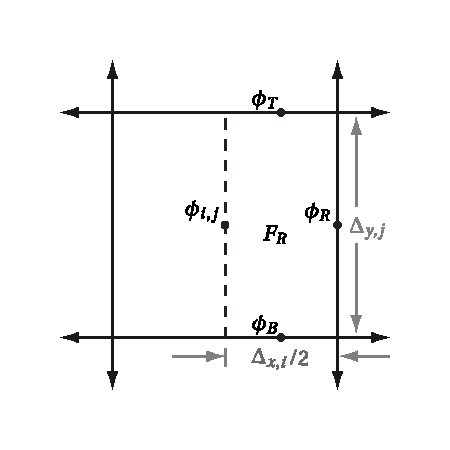
\includegraphics{goldin-righthalf}
  \caption{Right half of cell $i,j$.}
  \label{fig:goldinRight}
\end{figure}
evaluating the flux exiting the right face $F_R^x = \vec{F}\vd\vec{n}_R$.
\begin{align*}
\int_{y_{j-1/2}}^{y_{j+1/2}} \int_{x_{i}}^{x_{i+1/2}}
\vec{n}_R \vd \vec{F}
\ud x \ud y
&=
\int_{y_{j-1/2}}^{y_{j+1/2}} \int_{x_{i}}^{x_{i+1/2}}
-\vec{n}_R \vd \Dtens \vd \grad \phi
\ud x \ud y
\\
F_R^x \frac{\Delta_{x,i} \Delta_{y,j}}{2}
&=
-
\begin{bmatrix}
  1 & 0
\end{bmatrix}
\begin{bmatrix}
  D_{i,j}^{xx} & D_{i,j}^{yx} \\
  D_{i,j}^{xy} & D_{i,j}^{yy}
\end{bmatrix}
\int_{y_{j-1/2}}^{y_{j+1/2}} \int_{x_{i}}^{x_{i+1/2}}
\begin{bmatrix}
  \tpder{\phi}{x} \\
  \tpder{\phi}{y}
\end{bmatrix}
\ud x \ud y
\\
F_R^x \frac{\Delta_{x,i} \Delta_{y,j}}{2}
&=
-
\begin{bmatrix}
  D_{i,j}^{xx} & D_{i,j}^{yx}
\end{bmatrix}
\begin{bmatrix}
  \left( \phi_R - \phi_{i,j} \right) \Delta_{y,j} \\
  \left( \phi_T - \phi_B \right) \Delta_{x,i} / 2
\end{bmatrix}
\ud x \ud y
\\
F_R^x
&= 
- D_{i,j}^{xx} \frac{\phi_R - \phi_{i,j}}{ \Delta_{x,i} / 2}
- D_{i,j}^{yx} \frac{\phi_T - \phi_B}{ \Delta_{y,j} }\ \,.
\end{align*}
Performing the same procedure for the left side, we obtain
\begin{align*}
\int_{y_{j-1/2}}^{y_{j+1/2}} \int_{x_{i-1/2}}^{x_{i}}
\vec{n}_L \vd \vec{F}
\ud x \ud y
&=
\int_{y_{j-1/2}}^{y_{j+1/2}} \int_{x_{i-1/2}}^{x_{i}}
-\vec{n}_L \vd \Dtens \vd \grad \phi
\ud x \ud y
\\
-F_L^x \frac{\Delta_{x,i} \Delta_{y,j}}{2}
&=
-
\begin{bmatrix}
  -1 & 0
\end{bmatrix}
\begin{bmatrix}
  D_{i,j}^{xx} & D_{i,j}^{yx} \\
  D_{i,j}^{xy} & D_{i,j}^{yy}
\end{bmatrix}
\int_{y_{j-1/2}}^{y_{j+1/2}} \int_{x_{i-1/2}}^{x_{i}}
\begin{bmatrix}
  \tpder{\phi}{x} \\
  \tpder{\phi}{y}
\end{bmatrix}
\ud x \ud y
\\
F_L^x \frac{\Delta_{x,i} \Delta_{y,j}}{2}
&=
-
\begin{bmatrix}
  D_{i,j}^{xx} & D_{i,j}^{yx}
\end{bmatrix}
\begin{bmatrix}
  \left( \phi_{i,j} - \phi_L \right) \Delta_{y,j} \\
  \left( \phi_T - \phi_B \right) \Delta_{x,i} / 2
\end{bmatrix}
\ud x \ud y
\\
F_L^x
&= 
- D_{i,j}^{xx} \frac{\phi_{i,j} - \phi_L}{ \Delta_{x,i} / 2}
- D_{i,j}^{yx} \frac{\phi_T - \phi_B}{ \Delta_{y,j} }\,.
\end{align*}

Rotating the coordinate system by swapping $x\leftrightarrow y$, $T
\leftrightarrow R$, $B \leftrightarrow L$, and $i \leftrightarrow j$, we have
corresponding equations for the top and bottom leakage terms:
\begin{align*}
F_T^y
&= 
- D_{i,j}^{yy} \frac{\phi_T - \phi_{i,j}}{ \Delta_{y,j} / 2}
- D_{i,j}^{xy} \frac{\phi_R - \phi_L}{ \Delta_{x,i} }\,,
\\  
F_B^y
&= 
- D_{i,j}^{yy} \frac{\phi_{i,j} - \phi_B}{ \Delta_{y,j} / 2}
- D_{i,j}^{xy} \frac{\phi_R - \phi_L}{ \Delta_{x,i} }\,.
\end{align*}

At each interior face, we demand that the scalar intensity $\phi$ is continuous,
i.e.,
\begin{equation*}
  \phi_{R,i,j} = \phi_{L,i+1,j} \equiv \phi_{i+1/2,j}\,.
\end{equation*}
Substituting these definitions and the net leakage expressions into the
conservation equation~\eqref{eq:ssConservationDisc}, we obtain $I\times J$
equations,
\begin{multline*}
- \Delta_{x,i} D_{i,j}^{yy}\frac{\phi_{i,j+1/2} - \phi_{i,j}}{\Delta_{y,j} / 2}
- \Delta_{x,i} D_{i,j}^{xy}\frac{\phi_{i+1/2,j} - \phi_{i-1/2,j}}{\Delta_{x,i} }
\\
+ \Delta_{x,i} D_{i,j}^{yy}\frac{\phi_{i,j} - \phi_{i,j-1/2}}{\Delta_{y,j} / 2}
+ \Delta_{x,i} D_{i,j}^{xy}\frac{\phi_{i+1/2,j} - \phi_{i-1/2,j}}{\Delta_{x,i} }
\\
- \Delta_{y,j} D_{i,j}^{xx}\frac{\phi_{i+1/2,j} - \phi_{i,j}}{\Delta_{x,i} / 2}
- \Delta_{y,j} D_{i,j}^{yx}\frac{\phi_{i,j+1/2} - \phi_{i,j-1/2}}{\Delta_{y,j} }
\\
+ \Delta_{y,j} D_{i,j}^{xx}\frac{\phi_{i,j} - \phi_{i-1/2,j}}{\Delta_{x,i} / 2}
+ \Delta_{y,j} D_{i,j}^{yx}\frac{\phi_{i,j+1/2} - \phi_{i,j-1/2}}{\Delta_{y,j} }
\\
+ \Delta_{x,i}\Delta_{y,j} \sigma_{a,i,j} \phi_{i,j}
= \Delta_{x,i}\Delta_{y,j} q_{i,j}\,.
\end{multline*}
The transverse leakage terms cancel, leaving
\begin{multline*}
\phi_{i,j} \left(
   4 D_{i,j}^{xx} \frac{\Delta_{y,j}}{\Delta_{x,i}}
 + 4 D_{i,j}^{yy} \frac{\Delta_{x,i}}{\Delta_{y,j}}
 + \Delta_{x,i}\Delta_{y,j} \sigma_{a,i,j} \right)
 \\
- 2 D_{i,j}^{xx} \frac{\Delta_{y,j}}{\Delta_{x,i}}
  \left( \phi_{i+1/2,j} + \phi_{i-1/2,j} \right)
- 2 D_{i,j}^{yy} \frac{\Delta_{x,i}}{\Delta_{y,j}}
  \left( \phi_{i,j+1/2} + \phi_{i,j-1/2} \right)
\\= \Delta_{x,i}\Delta_{y,j} q_{i,j}\,.
\end{multline*}

To complete the equations for the Gol'din discretization, we enforce continuity
of the radiation flux on interior faces, setting $F_{T,i,j}^y = F_{B,i,j+1}^y$
and $F_{R,i,j}^x = F_{L,i+1,j}^x$, to yield the relations
\begin{equation*}
- D_{i,j}^{yy} \frac{\phi_{i,j+1/2} - \phi_{i,j}}{ \Delta_{y,j} / 2}
- D_{i,j}^{xy} \frac{\phi_{i+1/2,j} - \phi_{i-1/2,j}}{ \Delta_{x,i} }
=
- D_{i,j+1}^{yy} \frac{\phi_{i,j+1} - \phi_{i,j+1/2}}{ \Delta_{y,j} / 2}
- D_{i,j+1}^{xy} \frac{\phi_{i+1/2,j+1} - \phi_{i-1/2,j+1}}{ \Delta_{x,i} }\,.
\end{equation*}
and
\begin{equation*}
- D_{i,j}^{xx} \frac{\phi_{i+1/2,j} - \phi_{i,j}}{ \Delta_{x,i} / 2}
- D_{i,j}^{yx} \frac{\phi_{i,j+1/2} - \phi_{i,j-1/2}}{ \Delta_{y,j} }
=
- D_{i+1,j}^{xx} \frac{\phi_{i+1,j} - \phi_{i,j}}{ \Delta_{x,i} / 2}
- D_{i+1,j}^{yx} \frac{\phi_{i+1,j+1/2} - \phi_{i+1,j-1/2}}{ \Delta_{y,j} }\,.
\end{equation*}

Note that, if $D^{xy} = D^{yx}=0$, the cell-edged $\phi$ can be eliminated
without approximation, and
Gol'din's method will reduce to the simple cell-centered difference scheme of
\S\ref{sec:discreteDiag}.

%%%%%%%%%%%%%%%%%%%%%%%%%%%%%%%%%%%%%%%%%%%%%%%%%%%%%%%%%%%%%%%%%%%%%%%%%%%%%%%%
\section{Nine-point stencil}

Fig.~\ref{fig:cellAnisoLeakage} shows the leakage out of cell $i,j$ through the
right face.
\begin{figure}[htb]
  \centering
  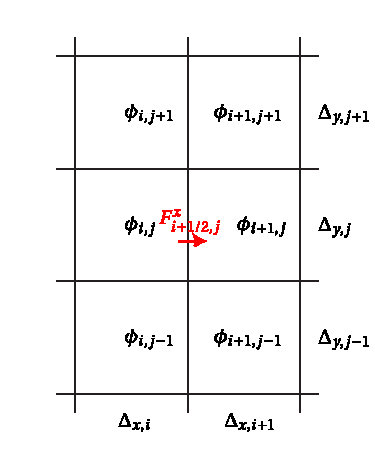
\includegraphics{cell-leakage-right}
  \caption{Diagram showing the radiation exiting interior cell $i,j$ through the
  right face.}
  \label{fig:cellAnisoLeakage}
\end{figure}
We evaluate the face-averaged normal component of the flux,
$F_{i+1/2,j}^x \equiv \int_{y_{j-1/2}}^{y_{j+1/2}} \vec{F} \vd \vec{n} \ud
y$, from both cell $i,j$ and cell $i+1,j$, and set them equal to each other.
Solving for $F_{i+1/2,j}^x$ gives
\begin{equation} \label{eq:cellAnisoFlux}
  F_{i+1/2,j}^{x} \approx
  - \frac{D^{xx}_{i+1/2,j}}{\Delta_{x,i+1/2}}
  \left[ 
    \left( \phi_{i+1,j} - \phi_{i,j} \right)
  + \frac{D^{xy}_{i,j}/D^{xx}_{i,j}}{2/\Delta_{x,i}}
    \pder{\phi}{y} \Bigg|_{x_{i+1/2}^-}
  + \frac{D^{xy}_{i+1,j}/D^{xx}_{i+1,j}}{2/\Delta_{x,i+1}}
    \pder{\phi}{y} \Bigg|_{x_{i+1/2}^+}
  \right]
\end{equation}
where $\tpder{\phi}{y} |_{x_{i+1/2}^-}$ is the transverse derivative of
$\phi$ on the left side of the face, and $\tpder{\phi}{y} |_{x_{i+1/2}^+}$ is
the transverse derivative as viewed from the right side of the face.
The harmonic-averaged diffusion coefficient is
\begin{equation} \label{eq:cellEdgeDHarmonic}
  \frac{D^{xx}_{i+1/2,j}}{\Delta_{x,i+1/2}} \equiv \left[
  \frac12 \left( \frac{D^{xx}_{i,j}}{\Delta_{x,i}} \right)\inv
 + \frac12 \left( \frac{D^{xx}_{i+1,j}}{\Delta_{x,i+1}} \right)\inv
  \right]\inv\,.
\end{equation}

If $D^{xy}$ were zero for both cells, and $D^{xx}=D^{yy}$,
Eq.~\eqref{eq:cellAnisoFlux} would reduce to
the standard cell-centered finite difference discretization so well known to
nuclear engineering students.

Now, in our first nine-point stencil, we approximated
\begin{equation*}
  \pder{\phi}{y} \Bigg|_{x_{i+1/2}^-} \approx \frac{\phi_{i,j+1} -
  \phi_{i,j-1}}{\tfrac12 \Delta_{y,j+1} + \Delta_{y,j} + \tfrac12
  \Delta_{y,j-1}}
\end{equation*}
in the interior of the problem and discarded the term near the boundaries. (The 
$\tpder{\phi}{y} |_{x_{i+1/2}^+}$ term is the same but replacing $i\to i+1$.)
An improvement is to approximate the case on the top boundary with
\begin{equation*}
  \pder{\phi}{y} \Bigg|_{x_{i+1/2}^-} \approx \frac{\phi_{i,j} -
  \phi_{i,j-1}}{\tfrac12 \Delta_{y,j} + \tfrac12 \Delta_{y,j-1} }
\end{equation*}
and the case on the bottom boundary with 
\begin{equation*}
  \pder{\phi}{y} \Bigg|_{x_{i+1/2}^-} \approx \frac{\phi_{i,j+1} -
  \phi_{i,j}}{\tfrac12 \Delta_{y,j+1} + \tfrac12 \Delta_{y,j} }
\end{equation*}

We can also approximate this derivative with approximate cell-edge values. In
the finite difference method, an intermediate cell-edge $\phi$ helps represent
the slope normal to the edge. It is eliminated in the process of finding
$\vec{F}\vd\vec{n}$, but if there is no transverse term, it is possible to
solve for the cell-edge $\phi$ in terms of the two cell-centered $\phi$. Let us
consider the finite difference approximation coupling two cells:
\begin{equation*}
  F = - D_0 \frac{\phi_{1/2} - \phi_0}{\Delta_0/2}
  \qquad\text{and}\qquad
  F = - D_1 \frac{\phi_{1} - \phi_{1/2}}{\Delta_1/2}\,.
\end{equation*}
Multiplying the left equation by $\Delta_0 / D_0$ and the right equation by
$\Delta_1 / D_1$,
\begin{equation*}
  -\frac{\Delta_0/2}{D_0 } F = \phi_{1/2} - \phi_0
  \qquad\text{and}\qquad
  -\frac{\Delta_1/2}{D_1 } F = \phi_{1} - \phi_{1/2}
\end{equation*}
adding them eliminates gives the standard finite-difference approximation for
$F$,
\begin{equation*}
  F = - \left( \frac{\Delta_0/2}{D_0 } + \frac{\Delta_1/2}{D_1 } \right)\inv
  \left( \phi_1 - \phi_0 \right),
\end{equation*}
and subtracting the second from the first gives
\begin{equation*}
 -\frac{\Delta_0/2}{D_0 }F + \frac{\Delta_1/2}{D_1 } F
 = 2 \phi_{1/2}-(\phi_0+\phi_1)\,.
\end{equation*}
Defining $ d_i \equiv \frac{\Delta_i}{D_i}$ for $i=0,1$ for brevity, then
\begin{equation*}
  \frac12 F (d_1 - d_0)
 = 2 \phi_{1/2}-(\phi_0+\phi_1)
  \qquad\text{and}\qquad
 F = -2\left( d_1 + d_0 \right)\inv (\phi_1 - \phi_0)\,.
\end{equation*}
Substituting $F$ into the left equation,
\begin{align*}
  \left( d_1 + d_0 \right)\inv\left(d_1 - d_0\right) (\phi_1 - \phi_0)
  &= 2 \phi_{1/2}-(\phi_0+\phi_1)
  \\
 \frac12 \left[ 1 - \frac{d_1 - d_0}{d_1 + d_0} \right] \phi_1
+ \frac12 \left[ 1 + \frac{d_1 - d_0}{d_1 + d_0} \right] \phi_0
 &= \phi_{1/2}
  \\
 \frac{d_0}{d_1 + d_0} \phi_1
+ \frac{d_1}{d_1 + d_0} \phi_0
 &= \phi_{1/2}\,.
\end{align*}

For our case in anisotropic diffusion, we want to approximate 
\begin{equation*}
  \pder{\phi}{y} \Bigg|_{x_{i+1/2}^-} \approx \frac{\phi_{i,j+1/2} -
  \phi_{i,j-1/2}}{\Delta_{y,j}} \,.
\end{equation*}
In evaluating these cell-edge $\phi$ we neglect the transverse leakage (as
leaving them in would add unknowns on more cell faces) and apply the previous
result:
\begin{equation*}
  \phi_{i,j+1/2} \approx
  \frac{D_{i,j}^{yy} / \Delta_{y,j}}{D_{i,j+1}^{yy} / \Delta_{y,j+1} +
  D_{i,j}^{yy} / \Delta_{y,j}} \phi_{i,j+1}
+ \frac{D_{i,j+1}^{yy} / \Delta_{y,j+1}}{D_{i,j+1}^{yy} / \Delta_{y,j+1} +
D_{i,j}^{yy} / \Delta_{y,j}} \phi_{i,j} \,.
\end{equation*}
Subtracting one from the $j$ indices gives the corresponding equation for the
bottom face:
\begin{equation*}
  \phi_{i,j-1/2} \approx
  \frac{D_{i,j-1}^{yy} / \Delta_{y,j-1}}{D_{i,j}^{yy} / \Delta_{y,j} +
  D_{i,j-1}^{yy} / \Delta_{y,j-1}} \phi_{i,j}
+ \frac{D_{i,j}^{yy} / \Delta_{y,j}}{D_{i,j}^{yy} / \Delta_{y,j} +
D_{i,j-1}^{yy} / \Delta_{y,j-1}} \phi_{i,j-1} \,.
\end{equation*}
If cell $i,j$ is in the interior, 
\begin{equation*}
  \pder{\phi}{y} \Bigg|_{x_{i+1/2}^-} \approx \frac{\phi_{i,j+1/2} -
  \phi_{i,j-1/2}}{\Delta_{y,j}} \,,
\end{equation*}
or if it is on the top boundary,
\begin{equation*}
  \pder{\phi}{y} \Bigg|_{x_{i+1/2}^-} \approx \frac{\phi_{i,j} -
  \phi_{i,j-1/2}}{\Delta_{y,j} / 2} \,,
\end{equation*}
or if it is on the bottom boundary,
\begin{equation*}
  \pder{\phi}{y} \Bigg|_{x_{i+1/2}^-} \approx \frac{\phi_{i,j+1/2} -
  \phi_{i,j}}{\Delta_{y,j} / 2} \,.
\end{equation*}

If the anisotropic diffusion coefficients are homogeneous and the grid is
uniform, this expression for $\tpder{\phi}{y}$ is exactly equivalent to the
simpler one.

\begin{figure}[htb]
  \centering
  \subfloat[Diagonal-only anisotropic]{%
  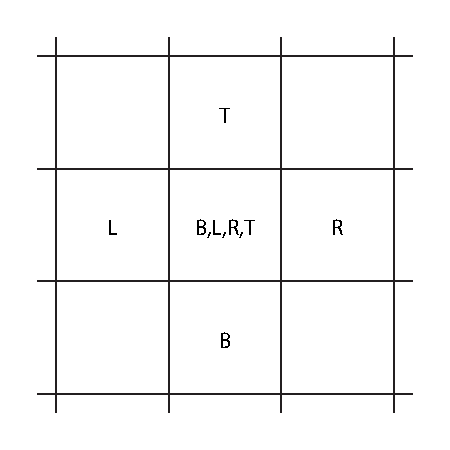
\includegraphics{diaganiso-leakage-terms}}
  \subfloat[Cell anisotropic]{%
  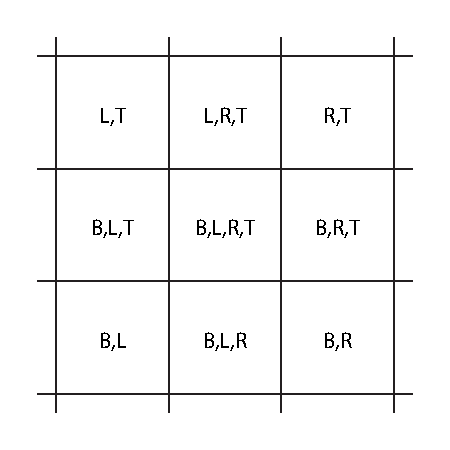
\includegraphics{cellaniso-leakage-terms}}
  \caption{Stencils for $- \grad \vd \Dtens \grad \phi$ showing contribution
  from the leakage terms of each face of the center cell.}
  \label{fig:anisoStencils}
\end{figure}

%%%%%%%%%%%%%%%%%%%%%%%%%%%%%%%%%%%%%%%%%%%%%%%%%%%%%%%%%%%%%%%%%%%%%%%%%%%%%%%%
\section{Incident boundary conditions} \label{sec:discreteBc}
(Do I show how to write boundary conditions for these schemes? I am sure that it
has been done before.)

For the cell-centered and staggered-mesh schemes of AD and \APone, respectively,
we desire boundary conditions that relate cell-edge leakage $\vec{n}\vd\vec{F}$
to cell-centered scalar intensity $\phi$.

A reflecting boundary condition for the transport equation translates to an
``insulating'' boundary condition in the low-order diffusion equations. There
is zero net leakage at the exterior face, $\vec{n}\vd\vec{F}=0$.

Incident boundary conditions are more complicated.
We will take the general \Pone\ boundary condition case:
\begin{subequations} \label{eqs:discreteBc}
\begin{equation} \label{eq:discreteBcGeneral}
  \beta = \phi - \alpha\vec{n}\vd \vec{F}
\end{equation}
with
\begin{equation} \label{eq:discreteBcGeneralF}
  \vec{n} \vd \vec{F}
  = - \vec{n}\vd \Dtens \vd \grad \phi
  + \gamma \vec{n}\vd \Dtens \vd \vec{F}^{i}\,.
\end{equation}
\end{subequations}
Here, $\beta$ is the source term that results from a positive incident
radiation source, $\alpha$ is the extrapolation distance, and $\gamma$ is
related to the geometry but is zero for diffusion.

\begin{table}[htb]
  \centering
  \begin{tabular}{rccc}
\toprule
& $\beta$
& $\alpha$
& $\gamma$
\\ \midrule
2-D Marshak AD
& $4 F^-$
& $2/3$
& $0$
\\
2-D Transport AD
& $2\int_{\vec{\Omega}\vd \vec{n} < 0} W I^b \ud\Omega$
& $0.7104$
& $0$
\\
Flatland Marshak AD
& $\pi F^-$
& $\pi/2$
& $0$
\\
2-D Marshak \APone
& $4 F^-$
& $2/3$
& $3/c \Delta_t$
\\
Flatland Marshak \APone
& $\pi F^-$
& $\pi/2$
& $2/c \Delta_t$
\\ \bottomrule
  \end{tabular}
  \caption{Coefficients for the discretized boundary conditions.}
  \label{tab:discreteBcCoeffs}
\end{table}

First, we note that, in accordance with the derivation in \S\ref{sec:zeta}, the
off-diagonal components of $\Dtens$ are zero, so we do not need to consider
transverse leakage at the boundary face. Evaluating
Eq.~\eqref{eq:discreteBcGeneralF} at a cell $i,j$ on the right boundary, and
introducing a temporary cell-edge $\phi_{i+1/2,j}$ with which we approximate the
gradient,
\begin{align} \nonumber
  F_R^y 
  &= - D_{i,j}^{xx} \frac{\phi_{i+1/2,j} - \phi_{i,j}}{\Delta_{x,i} / 2}
  + \gamma D_{i,j}^{xx} F_{i+1/2,j}^{i} \,.
\\ 
\intertext{For brevity, we write this as}
\label{eq:discreteBcFBrief}
  F
  &= - D \frac{\phi^* - \phi}{\Delta / 2}
  + \gamma D \hat F \,,
\end{align}
where $\phi^*$ is the cell-edge scalar intensity, and $\hat F$ is the initial
condition for the net radiation flux on the right face.

Substituting into Eq.~\eqref{eq:discreteBcGeneral}, which at the right boundary
is
\begin{equation*}
  \beta
  = \phi_{i+1/2,j}
  - \alpha F_R^y
  = \phi^* - \alpha F \,,
\end{equation*}
we obtain the relation
\begin{equation*}
  \beta
  = \phi^*
  + \alpha D \frac{\phi^* - \phi}{\Delta / 2}
  - \alpha \gamma D \hat F \,.
\end{equation*}
A little manipulation gives
\begin{equation*}
  \phi^* = \left( 1 + \frac{\alpha D}{\Delta/2} \right)\inv \left( \beta
  + \frac{\alpha D}{\Delta/2} \phi + \alpha \gamma D \hat F
  \right)\,.
\end{equation*}
We use this result to eliminate $\phi^*$ from Eq.~\eqref{eq:discreteBcFBrief}:
\begin{align*}
  F
  &= - \frac{D}{\Delta / 2} \phi^* + \frac{D}{\Delta / 2}\phi
  + \gamma D \hat F
  \\
  F
  &= -\left(  \frac{\Delta}{2 D} + \alpha\right)\inv
  \left( \beta
  + \frac{2 \alpha D}{\Delta} \phi + \alpha \gamma D \hat F
  \right)
  + \frac{D}{\Delta / 2}\phi
  + \gamma D \hat F
  \\
  F
  &= -\left(  \frac{\Delta}{2 D} + \alpha\right)\inv \beta
  + \left[ 1 - \left(1 + \frac{\Delta}{2 \alpha D} \right)\inv \right]
  \left( \frac{2D}{\Delta} \phi + \gamma D \hat F \right) \,.
\end{align*}
Because of potential machine precision error for optically thin cells
($\eps \equiv \Delta / D$), it is better to implement
\begin{equation*}
  \left[ 1 - \left( 1 + \frac{\Delta}{2 \alpha D} \right)\inv  \right]
  \to \left[ \frac{\frac{\Delta}{2 \alpha D}}{1 + \frac{\Delta}{2 \alpha D}}
  \right]
  = \left[ \frac{\Delta}{2 \alpha D + \Delta} \right]\,.
\end{equation*}
The equation for the net leakage out of a boundary cell on the right is
therefore
\begin{equation} \label{eq:discreteBcRight}
  F
  = -\left(  \frac{\Delta}{2 D} + \alpha\right)\inv \beta
  + \left[ 2 \alpha D + \Delta \right]\inv
  \left( 2D \phi + \gamma \Delta D \hat F \right) \,.
\end{equation}
This equation is also valid (after redefining $D=D^{yy}$, etc.) on the top
boundary, because there the sign of the face normal vector is also positive, and
the gradient is approximated in the same way.

On the left and bottom boundaries, $\vec{n}\vd \vec{F}$ and the approximation to
$\grad \phi$ have changes in sign. With diffusion ($\gamma=0$), the two sign
changes cancel, but the extra term in the \APone\ equation for $\vec{F}$ means
that one of the signs is different from Eq.~\eqref{eq:discreteBcRight}. The net
leakage term in Eq.~\eqref{eq:discreteBcGeneralF} for the left boundary takes on
a negative sign because $\vec{n}=- \vec{n}_x$, and the finite difference
approximation to $\grad \phi$ is different:
\begin{align} \nonumber
  \vec{F}\vd \vec{n} &= -F_L^x 
  \\
  &= (-1) \left(
  - D_{i,j}^{xx} \frac{\phi_{i,j} - \phi_{i-1/2,j}}{\Delta_{x,i} / 2}
  + \gamma D_{i,j}^{xx} F_{i+1/2,j}^{i}\right) \,,
\\ 
\intertext{or in brief form,}
\nonumber
F &= D \frac{\phi^* - \phi}{\Delta / 2} - \gamma D \hat F \,.
\end{align}
The term with $\hat F$ has a different sign from the corresponding term on a
positive boundary. Substituting this expression into
Eq.~\eqref{eq:discreteBcGeneral} gives
\begin{equation*}
  \beta = \phi^*
  + \alpha D \frac{\phi^* - \phi}{\Delta / 2} + \alpha \gamma D \hat F \,.
\end{equation*}
Eliminating $\phi^*$ from the previous equation gives the net current on the
left face:
\begin{equation*}
  F
  = -\left(  \frac{\Delta}{2 D} + \alpha\right)\inv \beta
  + \left[ 2 \alpha D + \Delta \right]\inv
  \left( 2D \phi - \gamma \Delta D \hat F \right) \,.
\end{equation*}
This equation, valid for bottom and left boundaries, has the same sign as the
top and right for the $\phi$ term but the opposite sign for the $\hat F$ term.


